% https://tex.stackexchange.com/a/266113/173708
\documentclass[border=3mm,tikz]{standalone}
%\documentclass{article}
\usepackage{amsmath}
\usepackage{tikz}
\usetikzlibrary{matrix}

\newcommand\funsum{}
\newcommand\scell[2]{}
\newcommand\inmblue[1]{}

\colorlet{mlightgray}{lightgray}

\begin{document}
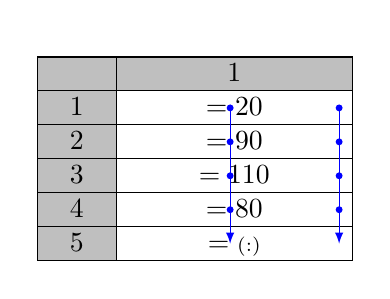
\begin{tikzpicture}[cell/.style={rectangle,draw=black}, nodes in empty cells]
  \matrix[
  matrix of math nodes,
  row sep =-\pgflinewidth,
  column sep = -\pgflinewidth,
  nodes={anchor=center, minimum width=2cm, cell},
  column 1/.style = {nodes={minimum width=1cm, fill=mlightgray}},
  column 2/.style = {nodes={minimum width=3cm}},
  row 1/.style = {nodes={text height=1.3ex, text depth=0, fill=mlightgray}},
  row 2/.style = {text height=1.3ex, text depth=0},
  row 3/.style = {text height=1.3ex, text depth=0},
  row 4/.style = {text height=1.3ex, text depth=0},
  row 5/.style = {text height=1.3ex, text depth=0},  
  row 6/.style = {text height=1.3ex, text depth=0},
  ] (m)
  {   &  \text{1}   \\
    \text{1} & =20  \\
    \text{2} & =90  \\
    \text{3} & =110 \\
    \text{4} & =80  \\
    \text{5} & = {\scriptstyle \funsum(\scell{1}{1}:\scell{4}{1})} \\
  };
  \node[font=\Large,anchor=south] at (m.north) {\inmblue{Formulas}};
  \draw[blue,-latex] 
    ([xshift=-1.5pt]m-2-2.center) -- ([xshift=-1.5pt]m-6-2.center); 
  \foreach \x in {2,...,5}
    {\fill[blue] ([xshift=-1.5pt]m-\x-2.center) circle (1.25pt);} 
  \draw[blue,-latex] 
    ([xshift=-5pt]m-2-2.east) -- ([xshift=-5pt]m-6-2.east); 
  \foreach \x in {2,...,5}
    {\fill[blue] ([xshift=-5pt]m-\x-2.east) circle (1.25pt);} 
\end{tikzpicture}

\end{document}